\documentclass[12pt]{article}%Imports
\usepackage{graphicx,abstract,epstopdf,times,authblk,geometry,fancyhdr,etoolbox,caption,sectsty,float}
\usepackage[sort,round]{natbib}

%Margins
\newgeometry{top=2cm,left=2.5cm,right=2.5cm,bottom=4.5cm}

%Header
\addtolength{\headheight}{1.5cm}
\pagestyle{fancyplain}
\lhead{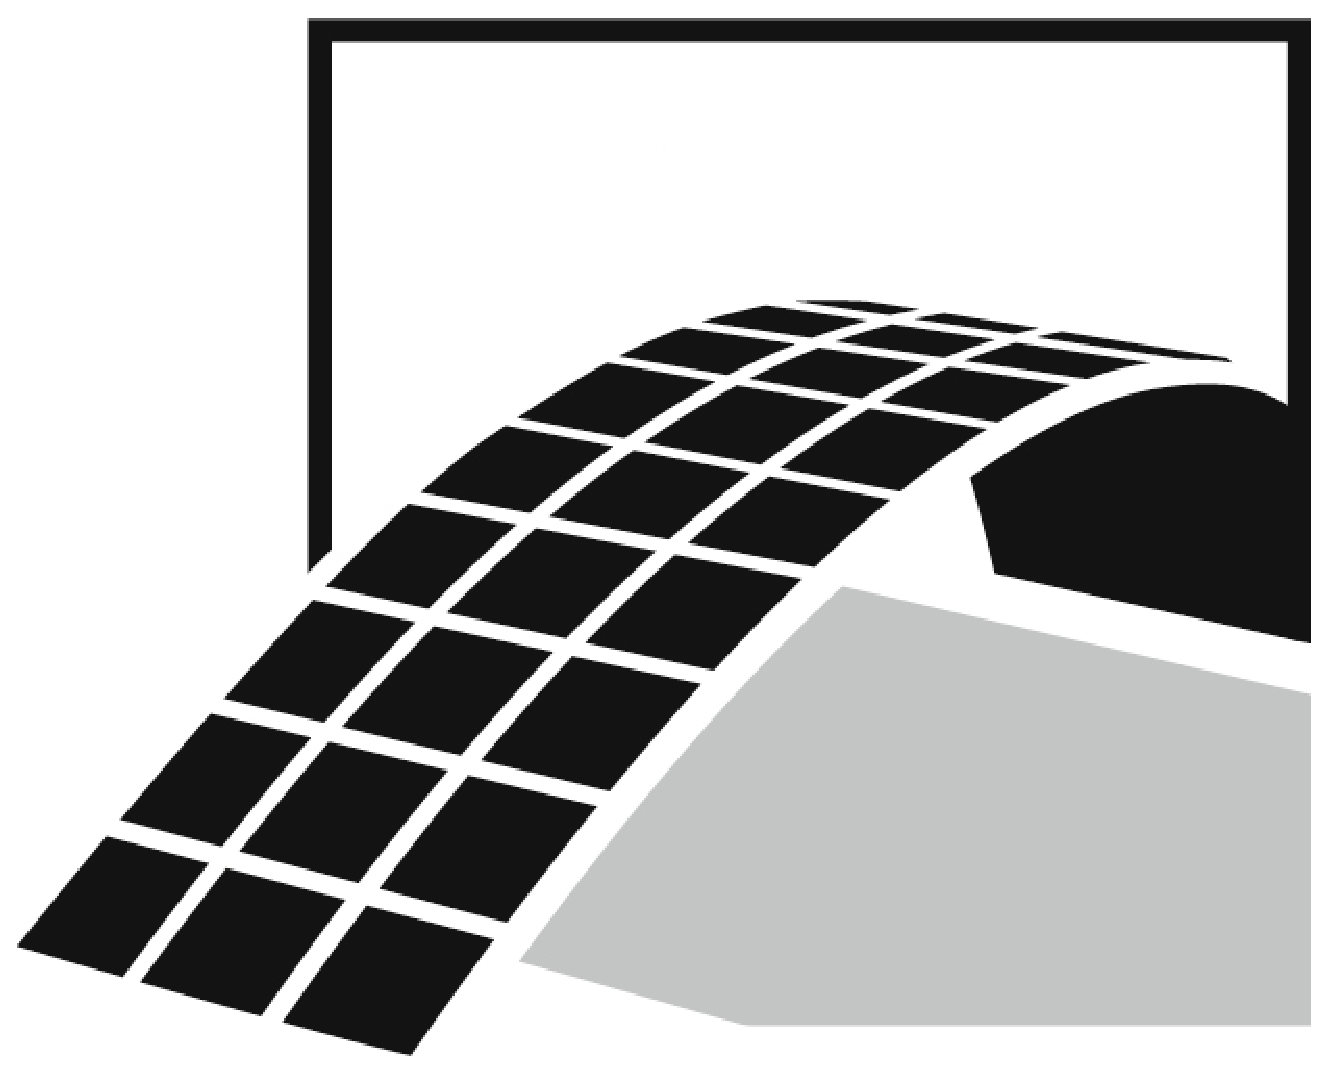
\includegraphics[height=1.3cm]{src/logo.eps} Chair of Computation in Engineering}
\rhead{Software-Lab 2016}
\renewcommand{\headrulewidth}{0pt}

%Layout
\renewcommand\Authfont{\fontsize{10pt}{9pt}\selectfont }
\renewcommand\Affilfont{\fontsize{10pt}{9pt}\selectfont }
\renewcommand\Authands{, }
\renewcommand{\abstractname}{\vspace{-\baselineskip}}
\renewcommand{\abstracttextfont}{\fontsize{10pt}{12pt}\selectfont\noindent\textbf{Abstract. }}
\date{\vspace{-\baselineskip}\vspace{-\baselineskip}}
\captionsetup{font=small}
\allsectionsfont{\fontsize{12pt}{14pt}\selectfont\bfseries }
\renewcommand{\arraystretch}{1.8}
\AtBeginEnvironment{tabular}{\fontsize{10pt}{9pt}\selectfont}
\bibliographystyle{src/agsm}
\newcommand\emails{\affil[ ]}


\title{Software-Lab Authors' Paper-Report}


%Add/Remove authors as you please
%Numbers in [] correspond to affiliations below
%\emails must be before \affils

\author[1]{Author A}
\author[1]{Author B}
\author[1]{Author C}   
\author[1]{Supervisor D}
\author[2]{Supervisor E}

\emails{A.A@university.edu, B.B@university.edu, C.C@university.edu, D.D@university.edu, E.E@company.com}

\affil[1]{Chair, University}
\affil[2]{Department, Company}





\begin{document}

\maketitle

\begin{abstract}The abstract should summarize the contents of the software-lab topic and should contain at least 70 at most 150 words. It should be set in 10-point font size and should be inset 1.0 cm from the right and left margins. There should be two blank (10-point) lines before and after the abstract. This document is in the required format...
\end{abstract}


\section{Introduction}
This file can be used as a template. In such a case, notice that at the left-hand side MS-Word provide a Navigation tool, which will allow you to know whether you are setting the right headings.\\

Please send a final \LaTeX and PDF file of your paper to your supervisors before the final presentation. The maximum length of the paper should not exceed 10 pages, including tables, figures and references. 

\section{Motivation (Poster)}
Students should also prepare a Poster as part of the final documentation. Please, remember that the poster is the first contact for the other students with your topic, should wake up their attention and guide them to the paper to get more information. Poster and paper are NOT the same document, but two different ways to present your results.

\section{Scope (Paper preparation)}

Please ensure that the margins of the page are set for: 3 cm at the top and 2.5cm at the bottom, right and left margins. The text should be justified to occupy the full line width, so that the right margin is not ragged, with words hyphenated as appropriate. As of 2007 MS-Word supports Auto-Hyphenation.
Use 10-point type for the name(s) of the author(s) and 10-point type for the address(es) and the abstract. For the main text, please use 12-point type and single-line spacing. The font style must be Times. Italic type may be used to emphasize words in running text. Bold type and underlining should be avoided. 

\subsection{Headings}

Headings should be capitalized (i.e., nouns, verbs, and all other words except articles, prepositions, and conjunctions should be set with an initial capital) and should, with the exception of the title, be aligned to the left. Words joined by a hyphen are subject to a special rule. If the first word can stand alone, the second word should be capitalized. The font sizes are given in Table \ref{table:example}.

\begin{table}
\begin{center}
\caption{Font sizes in Tables should be 10 point with the bold headings.}
\label{table:example}
\begin{tabular}{|c|c|c|} \hline
\textbf{Heading level} & \textbf{Example} & \textbf{Font size and style} \\ \hline 
Title (centered) & Lecture Notes... & 14 point, bold \\ \hline
1st-level heading & 1 Introduction & 12 point, bold \\ \hline
2nd-level heading & 2.1 Printing Area & 12 point, bold \\ \hline
3rd-level heading & Headings.  Text follows... & 12 point, bold \\ \hline
4th-level heading & Remark.  Text follows... & 10 point, italic \\ \hline
\end{tabular}
\end{center}
\end{table}

\subsection{Figures}
Figures should be numbered and should have a caption which should always be positioned under the figures, in contrast to the caption belonging to a table, which should always appear above the table. Please centre the captions between the margins and set them in 11-point type. 

\begin{figure}[!ht]
	\begin{center}
	\includegraphics[width=140mm]{figure1.eps}
	\caption{Sets and Relations of a Planning Process Model}
	\label{figure:example1}
	\end{center}
\end{figure}

Colour pictures should be displayed in grey-scale, unless they would be the result of simulations where colours have an extra meaning.

\begin{figure}[!ht]
	\begin{center}
	\includegraphics[width=140mm]{figure2.png}
	\caption{Twin-Tunnel Model}
	\label{figure:example2}
	\end{center}
\end{figure}

\subsection{Formulas}

Displayed equations or formulas are centered and set on a separate line (with an extra line or half-line space above and below). Displayed expressions should be numbered for reference. The numbers should be consecutive within each section or within the contribution, with numbers enclosed in parentheses and set on the right margin. 

\subsection{Program Code}

Program listings or program commands in the text are normally set in courier font point 9. However try to avoid “Copy-Paste” code, as they need a lot of space and usually are difficult to follow. Use in such a cases UML diagrams or pseudo-code.

\subsection{Citations and References}

The Harvard referencing style must be used, e.g. \citealp{Ashrae2005}. Another cite with parentheses \citep{Mawdesley2004}. The list of references is headed “References” and is not assigned a number in the decimal system of headings. The list should be set in small print and placed at the end of your contribution, in front of the appendix, if one exists. Please do not insert a page break before the list of references if the page is not completely filled

\section{Conclusions / Future work}

At the end of the paper be sure you summarize the work done and that you give some hints for a future extension of your topic. 

\bibliography{softwarelab}

\end{document}